\chapter{Evaluations} \label{ch:result}
The INTERACTION Dataset \footnote{https://interaction-dataset.com/} is used to compare the algorithms and models for tracking traffic participants. The dataset contains multiple scenarios in different locations, where each scenario consists of multiple traffic participants. Each traffic participant is identified by an ID for each scenario and each frame per 0.1s has a set of vehicles and their position. The x and y position of the vehicle is noted per time step. The initial state of the system is set using assignments \eqref{eq:initial}.
\begin{equation}
\label{eq:initial}
\begin{split}
x_0 &= zonotope([zeros(n), diag([1000;1000;10;10;10;10])])\\
w_k &= [0.1;0.1;0.4;0.4;0.1;0.1]\\
v_k &= [0.1;0.1]
\end{split}
\end{equation}

\section{Computation Time}
Figure \ref{fig:timegraph} shows that the estimation for Volume Minimization rises exponentially. Hence, the Volume Minimization method is not considered on the following parameters because, as seen from the graph, Volume Minimization requires vast time to compute the estimation, which makes it futile in the state estimation for collision avoidance system.

\begin{figure}
\label{fig:timegraph}
\centering
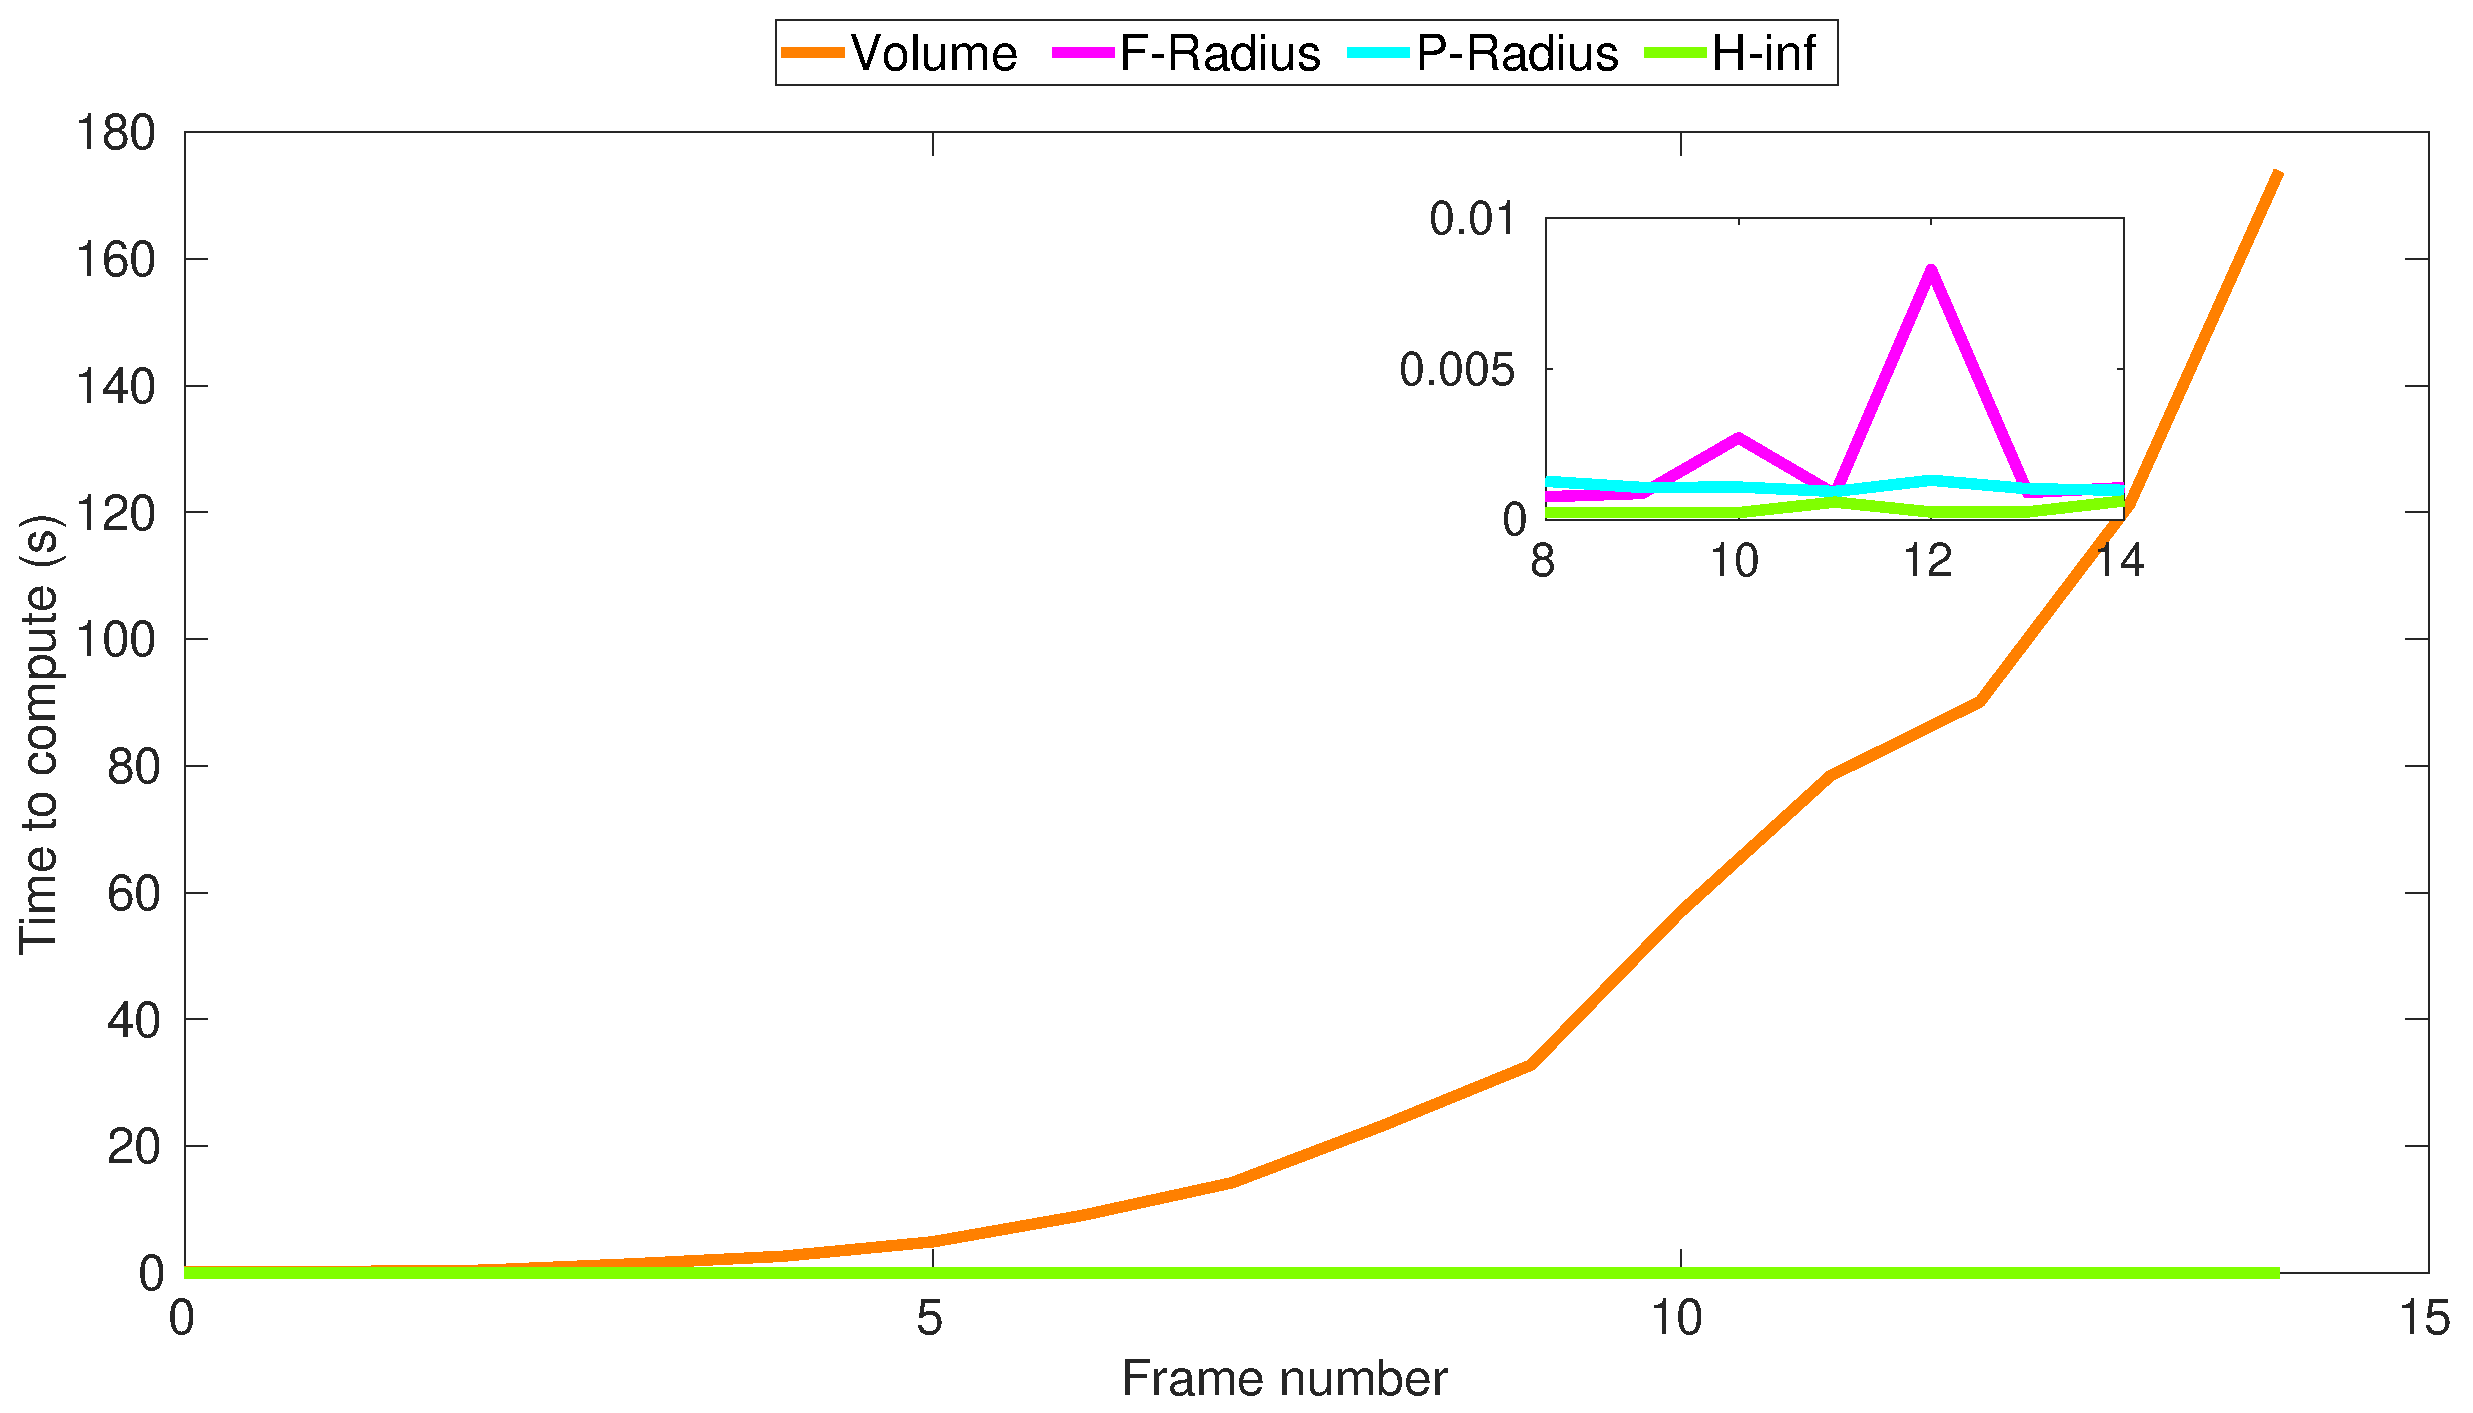
\includegraphics[width=.8\linewidth]{figures/timegraphh}
\caption{Computation time for each method}
\end{figure}

Average computation time for the segment intersection using F-Radius, P-Radius and interval observer using H-$\infty$ method for 10510 vehicles with cumulative 1623966 measurements of position in x and y-direction every 0.1s time step is tabulated in table \ref{tab:comptime}

\begin{table}[htbp]
\caption{Comparison of computation time(in ms) for 10510 vehicles in an intersection in USA\\}
	\centering
	\renewcommand{\arraystretch}{1.1}
	\small	
	\begin{tabular}{l l l l}
		\toprule 
		\textbf{Method} & \textbf{Constant Velocity} & \textbf{Constant Acceleration} & \textbf{Singer Acceleration} \\ \midrule
		%-------------------------------------		
		F-Radius & 0.396 & 0.375 & 0.399\\
		P-Radius & 0.312 & 0.319 & 0.317\\
		H-$\infty$ approximation & 0.145 & 0.147 & 0.142\\
		%--------------------------------------		
		\bottomrule
	\end{tabular}
	\label{tab:comptime}
\end{table}

\section{Time to Converge}
\begin{table}[htbp]
\caption{Comparison of average time(in ms) to converge for unmeasured state\\}
	\centering
	\renewcommand{\arraystretch}{1.1}
	\small	
	\begin{tabular}{l l l l}
		\toprule 
		\textbf{Method} & \textbf{Constant Velocity} & \textbf{Constant Acceleration} & \textbf{Singer Acceleration} \\ \midrule
		%-------------------------------------		
		F-Radius & 20 & 40 & 20\\
		P-Radius & 22 & 35 & 12\\
		H-$\infty$ approximation & 14 & 40 & 20\\
		%--------------------------------------		
		\bottomrule
	\end{tabular}
	\label{tab:convtime}
\end{table}

\section{Bounds}
\begin{table}[htbp]
\caption{Comparison of average time(in ms) to converge for unmeasured state\\}
	\centering
	\renewcommand{\arraystretch}{1.1}
	\small	
	\begin{tabular}{l l l l l l l}
		\toprule 
		& \multicolumn{6}{c}{\textbf{Constant Velocity}}\\
		\textbf{Method} & \textbf{$x$} & \textbf{$y$} & \textbf{$v_x$} & \textbf{$v_y$} & \textbf{$a_x$} & \textbf{$a_y$}\\ \midrule
		%-------------------------------------		
		F-Radius & .441 & .441 & 5.686 & 5.686 & - & -\\
		P-Radius & .4606 & .459 & 13.45 & 13.45 & - &	-\\
		H-$\infty$ approximation & .9867 &	.937 &	6.177 & 6.177 & - &-\\
		
		%--------------------------------------		
		
		& \multicolumn{6}{c}{\textbf{Constant Acceleration}}\\
		 & \textbf{$x$} & \textbf{$y$} & \textbf{$v_x$} & \textbf{$v_y$} & \textbf{$a_x$} & \textbf{$a_y$}\\ \midrule
		%-------------------------------------		
		F-Radius & .5713 &	.5075 &	8.461	& 8.461 &	15.86 &	15.97\\
		P-Radius & .4598 &	.4523 &	16.39 &	16.39 &	16.61 &	17.42\\
		H-$\infty$ approximation & 1.5 & 1.5 & 9.414 &	9.414 &	16.42 &	16.35\\
		
		%--------------------------------------		
		
		& \multicolumn{6}{c}{\textbf{Singer Acceleration}}\\
		 & \textbf{$x$} & \textbf{$y$} & \textbf{$v_x$} & \textbf{$v_y$} & \textbf{$a_x$} & \textbf{$a_y$}\\ \midrule
		%-------------------------------------		
		F-Radius &.4859	& .4859 &	7.38 & 7.383 &	11.53 &	11.53\\
		P-Radius & .7035 &	.7035 &	23.23 &	23.23 &	10.23 &	10.23\\
		H-$\infty$ approximation & 1.276 &	1.19 &	9.691 &	9.691 &	10.01 &	10.01\\
		\bottomrule
	\end{tabular}
	\label{tab:bound}
\end{table}


Time comparison for each method for n vehicles is shown in figure [cite]

As seen from Fig. \ref{fig:segmentminimization}, the upper and lower bounds of the state estimation by Segment Intersection(using Frobenius norm) of the system bounds the true state. Comparing the error in different states of the system, as shown in Fig. \ref{fig:comparison}, suggests that all the algorithms require around 1s to converge to near the true state. Interesting to note, the Interval Estimation has a higher error peak compared to Segment Minimization using the same dataset.\\

The Fig. \ref{fig:histogram} shows the Histogram of RMSE (Root Mean Square Error) of estimation from Segment Minimization. The errors are calculated after 10 seconds in order to avoid the initial peak. The histograms suggest that, the method gives little error for estimating the measured state, whereas, for unmeasured state like velocity, the error is at most twice the true state.


\begin{figure}[h!]
\begin{subfigure}{.5\textwidth}
\centering
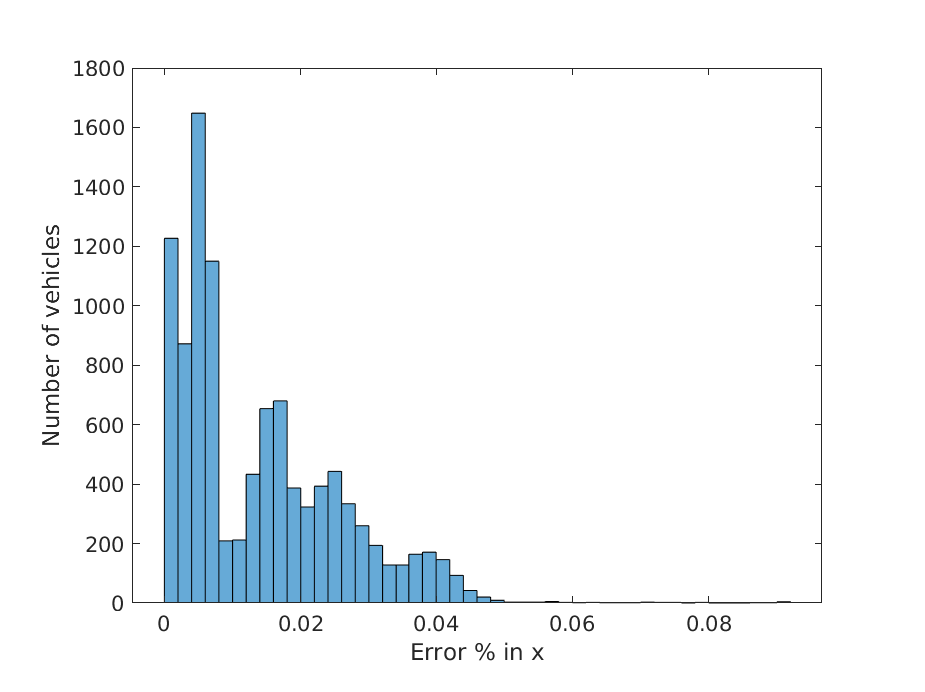
\includegraphics[width=.8\linewidth]{figures/s_caXerror}
\caption{RMSE $x$}
\end{subfigure}
\begin{subfigure}{.5\textwidth}
\centering
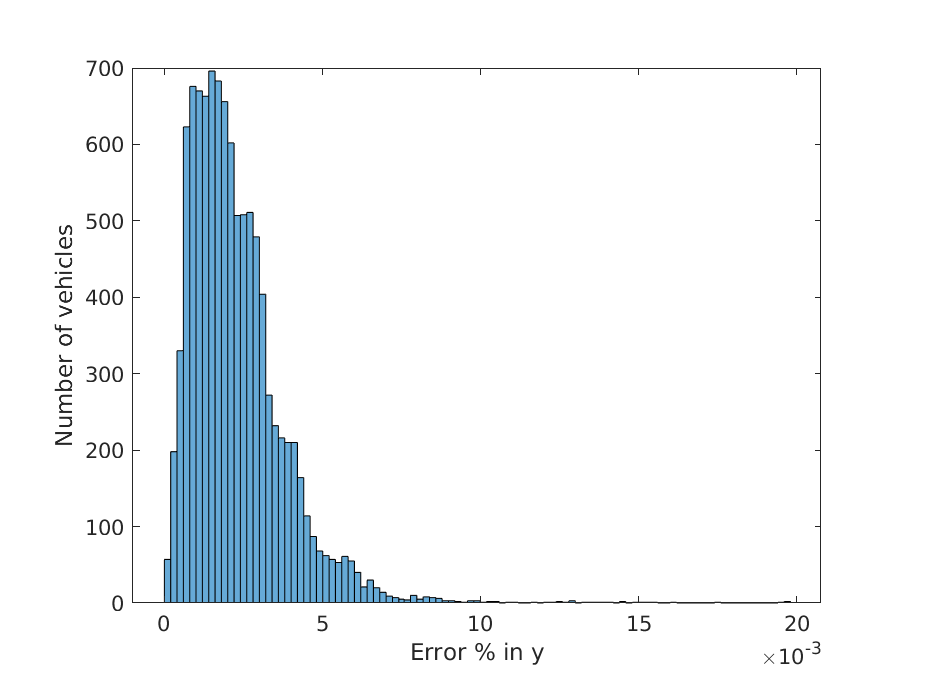
\includegraphics[width=.8\linewidth]{figures/s_caYerror}
\caption{RMSE $y$}
\end{subfigure}
\begin{subfigure}{.5\textwidth}
\centering
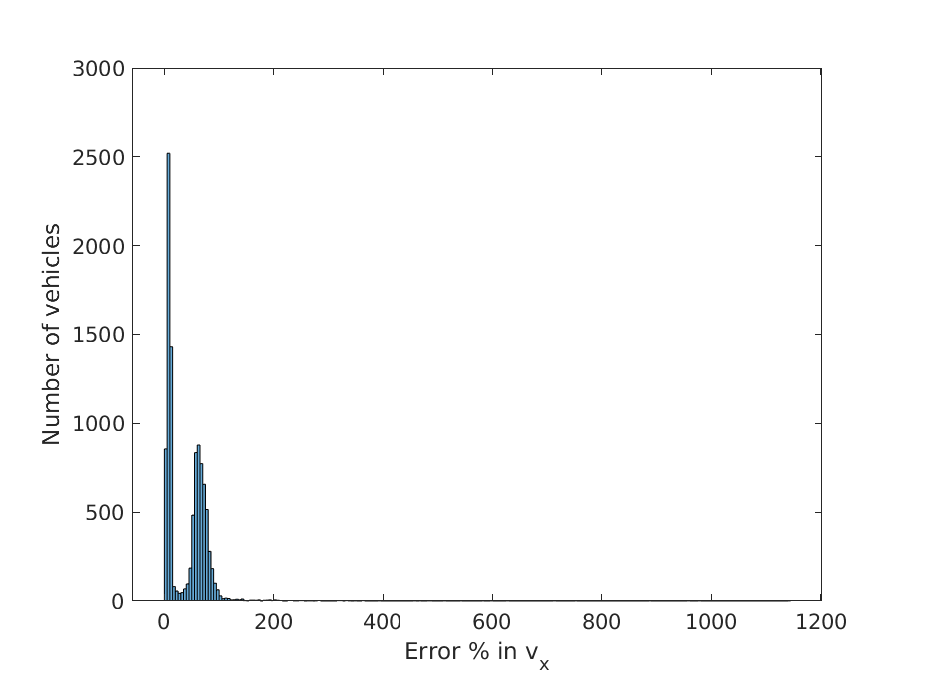
\includegraphics[width=.8\linewidth]{figures/s_cavXerror}
\caption{RMSE in $velocity_x$}
\end{subfigure}
\begin{subfigure}{.5\textwidth}
\centering
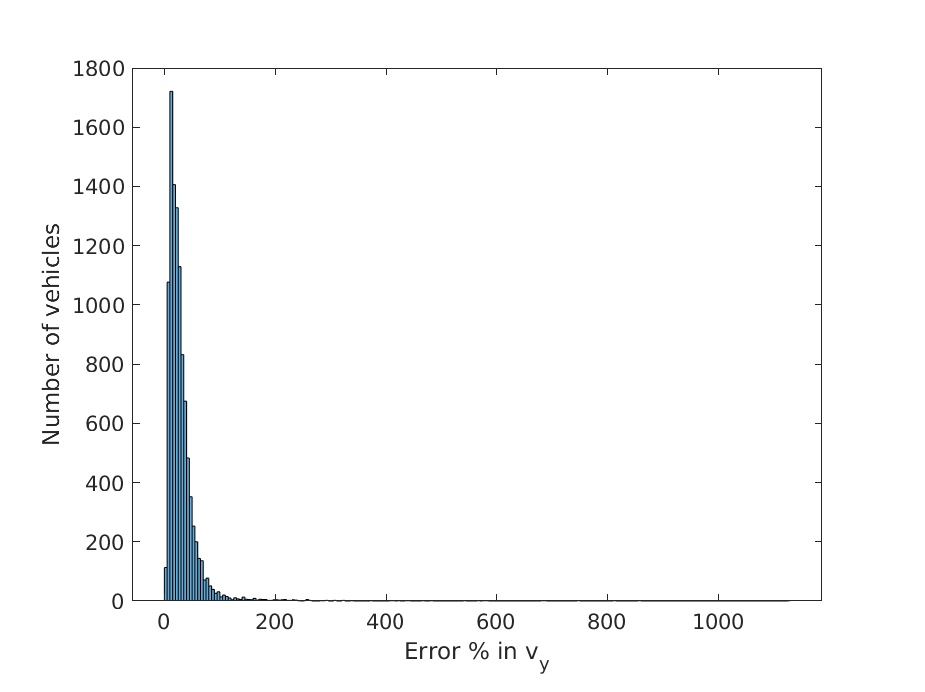
\includegraphics[width=.8\linewidth]{figures/s_cavYerror}
\caption{RMSE in $velocity_y$}
\end{subfigure}
\caption{Histogram of errors from Segment Minimizer on 651 vehicles }
\label{fig:histogram}
\end{figure}
%\begin{itemize}
%\item{Efficiency}
%\item{Accuracy}
%\item{Performance Metric}
